\documentclass[12pt,reqno]{amsart}
%\documentclass[../Solutions_Introduction_to_Algorithms.tex]{subfiles}
\usepackage{amsmath,amsfonts,amscd,amssymb,epsf,color,enumerate,graphicx,url}
\usepackage{algorithm, algorithmic}
\usepackage{forest, tikz, xcolor}
\usepackage{parskip}
\usetikzlibrary{matrix, positioning}
\setlength{\oddsidemargin}{-0.2in}%
\setlength{\evensidemargin}{-0.2in}%
\setlength{\textwidth}{6.6in}%
\setlength{\topmargin}{-0.5in}%
 \setlength{\textheight}{9.5in}%
 \definecolor{orange}{rgb}{1,0.5,0}
 \pagestyle{plain}
\linespread{1.3}
\usepackage[small]{caption}
\newcommand{\pa}{\partial}
\newcommand{\va}{\vspace{0.4cm}}
\newcommand{\di}{\displaystyle}
\newcommand{\disp}{\displaystyle}


% turn on \answertrue to show the solution
% turn on \answerfalse to hide the solution
\newif\ifanswer
\answertrue
%\answerfalse



\begin{document}
\noindent {\footnotesize Introduction to Algorithms}\hspace{10.5cm} {\footnotesize Solutions}

\vspace{0.5cm}
\hspace{5.5cm}\textbf{\large Exercises in Section 8.4}
\vspace{0.5cm}

\begin{enumerate}[1.]

\item Using Figure 8.4 as a model, illustrate the operation of \textsc{Bucket-Sort} on the array $A = \langle .79, .13, .16, .64, .39, .20, .89, .53, .71, .42 \rangle$.
\vspace{0.5cm}

\ifanswer
\noindent {\bf Solution}

I don't like Figure 8.4.
\begin{center}
    \begin{tikzpicture}
        \matrix[matrix of nodes,
                nodes={draw, minimum width=0.9cm, minimum height=0.9cm, anchor=center},
                column sep=0pt, row sep=0pt,
                name=m1] 
        {
            \node[fill=none, draw=none, name=m1-0-0] {~}; &
            \node[fill=none, draw=none, name=m1-0-1] {$A$}; &
            \node[fill=none, draw=none, name=m1-0-2] {~}; &
            \node[fill=none, draw=none, name=m1-0-3] {~}; &
            \node[fill=none, draw=none, name=m1-0-4] {$B$}; &
            \node[fill=none, draw=none, name=m1-0-5] {~}; &
            \node[fill=none, draw=none, name=m1-0-6] {~}; &
            \node[fill=none, draw=none, name=m1-0-7] {~}; &
            \node[fill=none, draw=none, name=m1-0-8] {~}; &
            \node[fill=none, draw=none, name=m1-0-9] {$B'$}; \\
            \node[fill=none, draw=none, name=m1-1-0] {1}; &
            \node[fill=pink,            name=m1-1-1] {.79}; & &
            \node[fill=none, draw=none, name=m1-1-2] {0}; &
            \node[fill=pink,            name=m1-1-3] {$\times$}; & & & & &
            \node[fill=pink,            name=m1-1-4] {$\times$}; \\
            \node[fill=none, draw=none, name=m1-2-0] {2}; &
            \node[fill=pink,            name=m1-2-1] {.13}; & &
            \node[fill=none, draw=none, name=m1-2-2] {1}; &
            \node[fill=pink,            name=m1-2-3] {.13}; &
            \node[fill=pink,            name=m1-2-4] {.16}; & & & &
            \node[fill=pink,            name=m1-2-5] {.13}; &
            \node[fill=pink,            name=m1-2-6] {.16}; \\
            \node[fill=none, draw=none, name=m1-3-0] {3}; &
            \node[fill=pink,            name=m1-3-1] {.16}; & &
            \node[fill=none, draw=none, name=m1-3-2] {2}; &
            \node[fill=pink,            name=m1-3-3] {.20}; & & & & &
            \node[fill=pink,            name=m1-3-4] {.20}; \\
            \node[fill=none, draw=none, name=m1-4-0] {4}; &
            \node[fill=pink,            name=m1-4-1] {.64}; & &
            \node[fill=none, draw=none, name=m1-4-2] {3}; &
            \node[fill=pink,            name=m1-4-3] {.39}; & & & & &
            \node[fill=pink,            name=m1-4-4] {.39}; \\
            \node[fill=none, draw=none, name=m1-5-0] {5}; &
            \node[fill=pink,            name=m1-5-1] {.39}; & &
            \node[fill=none, draw=none, name=m1-5-2] {4}; &
            \node[fill=pink,            name=m1-5-3] {.42}; & & &
            \node[fill=none, draw=none, name=m1-5-4] {$\longrightarrow$}; & &
            \node[fill=pink,            name=m1-5-5] {.42}; \\
            \node[fill=none, draw=none, name=m1-6-0] {6}; &
            \node[fill=pink,            name=m1-6-1] {.20}; & &
            \node[fill=none, draw=none, name=m1-6-2] {5}; &
            \node[fill=pink,            name=m1-6-3] {.53}; & & & & &
            \node[fill=pink,            name=m1-6-4] {.53}; \\
            \node[fill=none, draw=none, name=m1-7-0] {7}; &
            \node[fill=pink,            name=m1-7-1] {.89}; & &
            \node[fill=none, draw=none, name=m1-7-2] {6}; &
            \node[fill=pink,            name=m1-7-3] {.64}; & & & & &
            \node[fill=pink,            name=m1-7-4] {.64}; \\
            \node[fill=none, draw=none, name=m1-8-0] {8}; &
            \node[fill=pink,            name=m1-8-1] {.53}; & &
            \node[fill=none, draw=none, name=m1-8-2] {7}; &
            \node[fill=pink,            name=m1-8-3] {.79}; &
            \node[fill=pink,            name=m1-8-4] {.71}; & & & &
            \node[fill=pink,            name=m1-8-5] {.71}; &
            \node[fill=pink,            name=m1-8-6] {.79}; \\
            \node[fill=none, draw=none, name=m1-9-0] {9}; &
            \node[fill=pink,            name=m1-9-1] {.71}; & &
            \node[fill=none, draw=none, name=m1-9-2] {8}; &
            \node[fill=pink,            name=m1-9-3] {.89}; & & & & &
            \node[fill=pink,            name=m1-9-4] {.89}; \\
            \node[fill=none, draw=none, name=m1-10-0] {10}; &
            \node[fill=pink,            name=m1-10-1] {.42}; & &
            \node[fill=none, draw=none, name=m1-10-2] {9}; &
            \node[fill=pink,            name=m1-10-3] {$\times$}; & & & & &
            \node[fill=pink,            name=m1-10-4] {$\times$}; \\
        };
    \end{tikzpicture}\\
\end{center}
Note that the arrow means insertion sort on each row of $B$.

\vspace{1cm}



\item Explain why the worst-case running time for bucket sort is $\Theta(n^2)$. What simple change to the algorithm preserves its linear average-case running time and makes its worst-case running time $O(n\lg{n})$?
\vspace{0.5cm}

\ifanswer
\noindent {\bf Solution}

If, coincidentally, all $n$ elements fall in the same interval, say $B[0]$. Then, insertion sort on $B[0]$ would cost $\Theta(n^2)$ time.

To reduce the worst-case running time to $O(n\lg{n})$, we can simply replace insertion sort by other sorting methods that run in $O(n\lg{n})$ (e.g. merge sort, heapsort, quicksort).

\vspace{1cm}



\item Let $X$ be a random variable that is equal to the number of heads in two flips of a fair coin. What is $E[X^2]$? What is $E^2[X]$?
\vspace{0.5cm}

\ifanswer
\noindent {\bf Solution}

Note that $X$ follows binomial distribution. More precisely, $X \sim B(2, \frac{1}{2})$. Thus, $$ E[X] = 2\left(\frac{1}{2}\right) = 1, \quad\text{and}\quad \text{Var}[X] = 2\left(\frac{1}{2}\right)\left(1 - \frac{1}{2}\right) = \frac{1}{2}. $$ Therefore, $$ E^2[X] = 1^2 = 1, $$ and $$ E[X^2] = \text{Var}[X] + E^2[X] = \frac{1}{2} + 1 = \frac{3}{2}. $$

\vspace{1cm}



\item An array $A$ of size $n > 10$ is filled in the following way. For each element $A[i]$, choose two random variables $x_i$ and $y_i$ uniformly and independently from $[0, 1)$. Then set $$ A[i] = \frac{\lfloor 10x_i \rfloor}{10} + \frac{y_i}{n}. $$ Modify bucket sort so that it sorts the array $A$ in $O(n)$ expected time.
\vspace{0.5cm}

\ifanswer
\noindent {\bf Solution}

Modify line 5 from $$\text{insert $A[i]$ into list $B[\lfloor n \cdot A[i] \rfloor]$}$$ to $$\text{insert $A[i]$ into list $B[\lfloor \frac{n^2}{10} \cdot \left(10 \cdot A[i] - \lfloor 10 \cdot A[i] \rfloor\right) \rfloor]$},$$ where $10 \cdot A[i] - \lfloor 10 \cdot A[i] \rfloor$ is the decimal part of $$10 \cdot A[i] = \lfloor 10x_i \rfloor + \frac{10}{n}y_i.$$ It is easy to see the decimal part is exactly $\frac{10}{n}y_i$. Finally, $$\lfloor \frac{n^2}{10} \cdot \frac{10}{n}y_i \rfloor = \lfloor n \cdot y_i \rfloor.$$ Since $y_i$ varies uniformly in $[0, 1)$, it aligns exactly with classic bucket sort.
\vspace{1cm}



\item You are given $n$ points in the unit disk, $p_i = (x_i, y_i)$, such that $0 < x_i^2 + y_i^2 \leq 1$ for $i = 1, 2, \dots, n$. Suppose that the points are uniformly distributed, that is, the probability of finding a point in any region of the disk is proportional to the area of that region. Design an algorithm with an average-case running time of $\Theta(n)$ to sort the $n$ points by the distances $d_i = \sqrt{x_i^2 + y_i^2}$ from the origin. (\textit{Hint:} Design the bucket sizes in \textsc{Bucket-Sort} to reflect the uniform distribution of the points in the unit disk.)
\vspace{0.5cm}

\ifanswer
\noindent {\bf Solution}

Let $B[0]$ contain $p_i$ where $0 < d_1 \leq \frac{1}{\sqrt{n}}$, $B[1]$ contain $p_i$ where $\frac{1}{\sqrt{n}} < d_i \leq \frac{\sqrt{2}}{\sqrt{n}}$, $\dots$, $B[n - 1]$ contain $p_i$ where $\frac{\sqrt{n - 1}}{\sqrt{n}} < d_i \leq 1$. It is easy to check the areas of these regions are the same, yielding equal probability.
\vspace{1cm}



\item A \textit{\textbf{probability distribution function}} $P(x)$ for a random variable $X$ is defined by $P(x) = \text{Pr}\{X \leq x\}$. Suppose that you draw a list of $n$ random variables $X_1, X_2, \dots, X_n$ from a continuous probability distribution function $P$ that is computable in $O(1)$ time (given $y$ you can find $x$ such that $P(x) = y$ in $O(1)$ time). Given an algorithm that sorts these numbers in linear average-case time.
\vspace{0.5cm}

\ifanswer
\noindent {\bf Solution}

For each $i = 0, 1, \dots, n - 1$, let $y_i = \frac{i}{n}$, and find the corresponding $x_i$ in $O(1)$ time. The total time cost for this step is $O(n)$ (in addition, define $x_n = 1$). Then, apply bucket sort with buckets $\{[x_i, x_{i + 1})\}$, again in $O(n)$ time.
\vspace{1cm}




\end{enumerate}

\end{document}



